\documentclass{article}

\usepackage{tikz}
\usepackage{float}
\usepackage{multirow}
\usepackage{rotating}
\usepackage[margin=1in]{geometry}

\graphicspath{ {./images} }

\title{
    Manutenção Inteligente em Cenário de Indústria 4.0 \\
    \vspace{0.75em}
    \Large Entrega 2 \\  \vspace{1.25em} 
    \large
    \begin{tabular}{rl}
        \textbf{Turno:}& MODL03 \\ 
        \rule{0pt}{1.25em} 
        \textbf{Docente:}& Maria do Rosário Bernardo 
    \end{tabular}
}
\author{}
\date{}


\begin{document}
    \maketitle
    \begin{tikzpicture}[overlay, remember picture]
        \node[xshift=3.5cm,yshift=-2.5cm] at (current page.north west) {
\includegraphics[scale = 0.35]{logo_ist.jpeg}};
    \end{tikzpicture}
    \vspace{-1.2em}
    \begin{table}[H]
        \centering
        \begin{tabular}{|l|l|l|l|l}
        \cline{1-4}
        \multicolumn{1}{|l|}{}                   & \multicolumn{1}{l|}{}       & \multicolumn{1}{l|}{}                             & \multicolumn{1}{l|}{}                   &  \\
        \multicolumn{1}{|l|}{}                   & \multicolumn{1}{l|}{}       & \multicolumn{1}{l|}{}                             & \multicolumn{1}{l|}{}                   &  \\
        \multicolumn{1}{|c|}{Nome}               & \multicolumn{1}{c|}{Número} & \multicolumn{1}{c|}{Esforço estimado de trabalho} & \multicolumn{1}{c|}{Tarefas realizadas} &  \\
        \multicolumn{1}{|l|}{}                   & \multicolumn{1}{l|}{}       & \multicolumn{1}{l|}{}                             & \multicolumn{1}{l|}{}                   &  \\
        \multicolumn{1}{|l|}{}                   & \multicolumn{1}{l|}{}       & \multicolumn{1}{l|}{}                             & \multicolumn{1}{l|}{}                   &  \\ \cline{1-4}
        \multicolumn{1}{|l|}{}                   & \multicolumn{1}{l|}{}       & \multicolumn{1}{l|}{}                             & \multirow{5}{7cm}{Extração de atividades e eventos relevantes para a manutenção a partir do UoD. Modelação do processo de manutenção em BPMN.}                   &   \\
        \multicolumn{1}{|l|}{}                   & \multicolumn{1}{l|}{}       & \multicolumn{1}{l|}{}                             & \multicolumn{1}{l|}{}                   &  \\
        \multicolumn{1}{|c|}{Sebastião Assunção} & \multicolumn{1}{c|}{95536}  & \multicolumn{1}{c|}{12 horas}                     & \multicolumn{1}{l|}{}                   &  \\
        \multicolumn{1}{|l|}{}                   & \multicolumn{1}{l|}{}       & \multicolumn{1}{l|}{}                             & \multicolumn{1}{l|}{}                   &  \\
        \multicolumn{1}{|l|}{}                   & \multicolumn{1}{l|}{}       & \multicolumn{1}{l|}{}                             & \multicolumn{1}{l|}{}                   &  \\ \cline{1-4}
        \multicolumn{1}{|l|}{}                   & \multicolumn{1}{l|}{}       & \multicolumn{1}{l|}{}                             & \multirow{5}{7cm}{Modelação do processo de manutenção em BPMN. Representação da colaboração entre as entidades participantes na manutenção no diagrama com múltiplicas pools.}                   &  \\
        \multicolumn{1}{|l|}{}                   & \multicolumn{1}{l|}{}       & \multicolumn{1}{l|}{}                             & \multicolumn{1}{l|}{}                   &  \\
        \multicolumn{1}{|c|}{Duarte Almeida}     & \multicolumn{1}{c|}{95565}  & \multicolumn{1}{c|}{12 horas}                     & \multicolumn{1}{l|}{}                   &  \\
        \multicolumn{1}{|l|}{}                   & \multicolumn{1}{l|}{}       & \multicolumn{1}{l|}{}                             & \multicolumn{1}{l|}{}                   &  \\
        \multicolumn{1}{|l|}{}                   & \multicolumn{1}{l|}{}       & \multicolumn{1}{l|}{}                             & \multicolumn{1}{l|}{}                   &  \\ \cline{1-4}
        \end{tabular}
        \end{table}

    \vspace{0.3cm}

    \noindent \large \textbf{Comentários aos diagramas}

    \vspace{0.5em} \normalsize
    Os eventos de início do processo de manutenção, citados a partir do enunciado, foram numerados da seguinte forma:
    \vspace{-0.1em}
    \begin{itemize}
        \itemsep0em 
        \item[--] Evento de início 1: uaTEC regista nova versão de appCTR;
        \item[--] Evento de início 2: TWIN avisa de avaria identificada;
        \item[--] Evento de início 3: TWIN avisa de avaria inferida;
        \item[--] Evento de início 4: TWIN avisa de impossibilidade de se atingir um ponto de carregamento das baterias por distância excedida;
        \item[--] Evento de início 5: Avaria inferida porque não está a decorrer instalação da appCTR e a mesma não reportou nada dentro de intervalo de tempo para tal definido pelo fornecedor. 
    \end{itemize} \par
    \vspace{-0.1em}
    A condição (a) presente na lane (resp. pool) no diagrama 1 (resp. 2) é verdadeira se e só se a máquina estava a ser usada por arPRO quando o evento
    de início da primeira execução do processo foi gerado ou a máquina tem uso por arPRO previsto para as 24h seguintes. \par
    De referir ainda que todos os conectores de associação têm como destino a appMNG, tendo-se colapsado múltiplos conectores por razões de clareza visual.
    \pagebreak

    \begin{figure}[H]
        \centering
        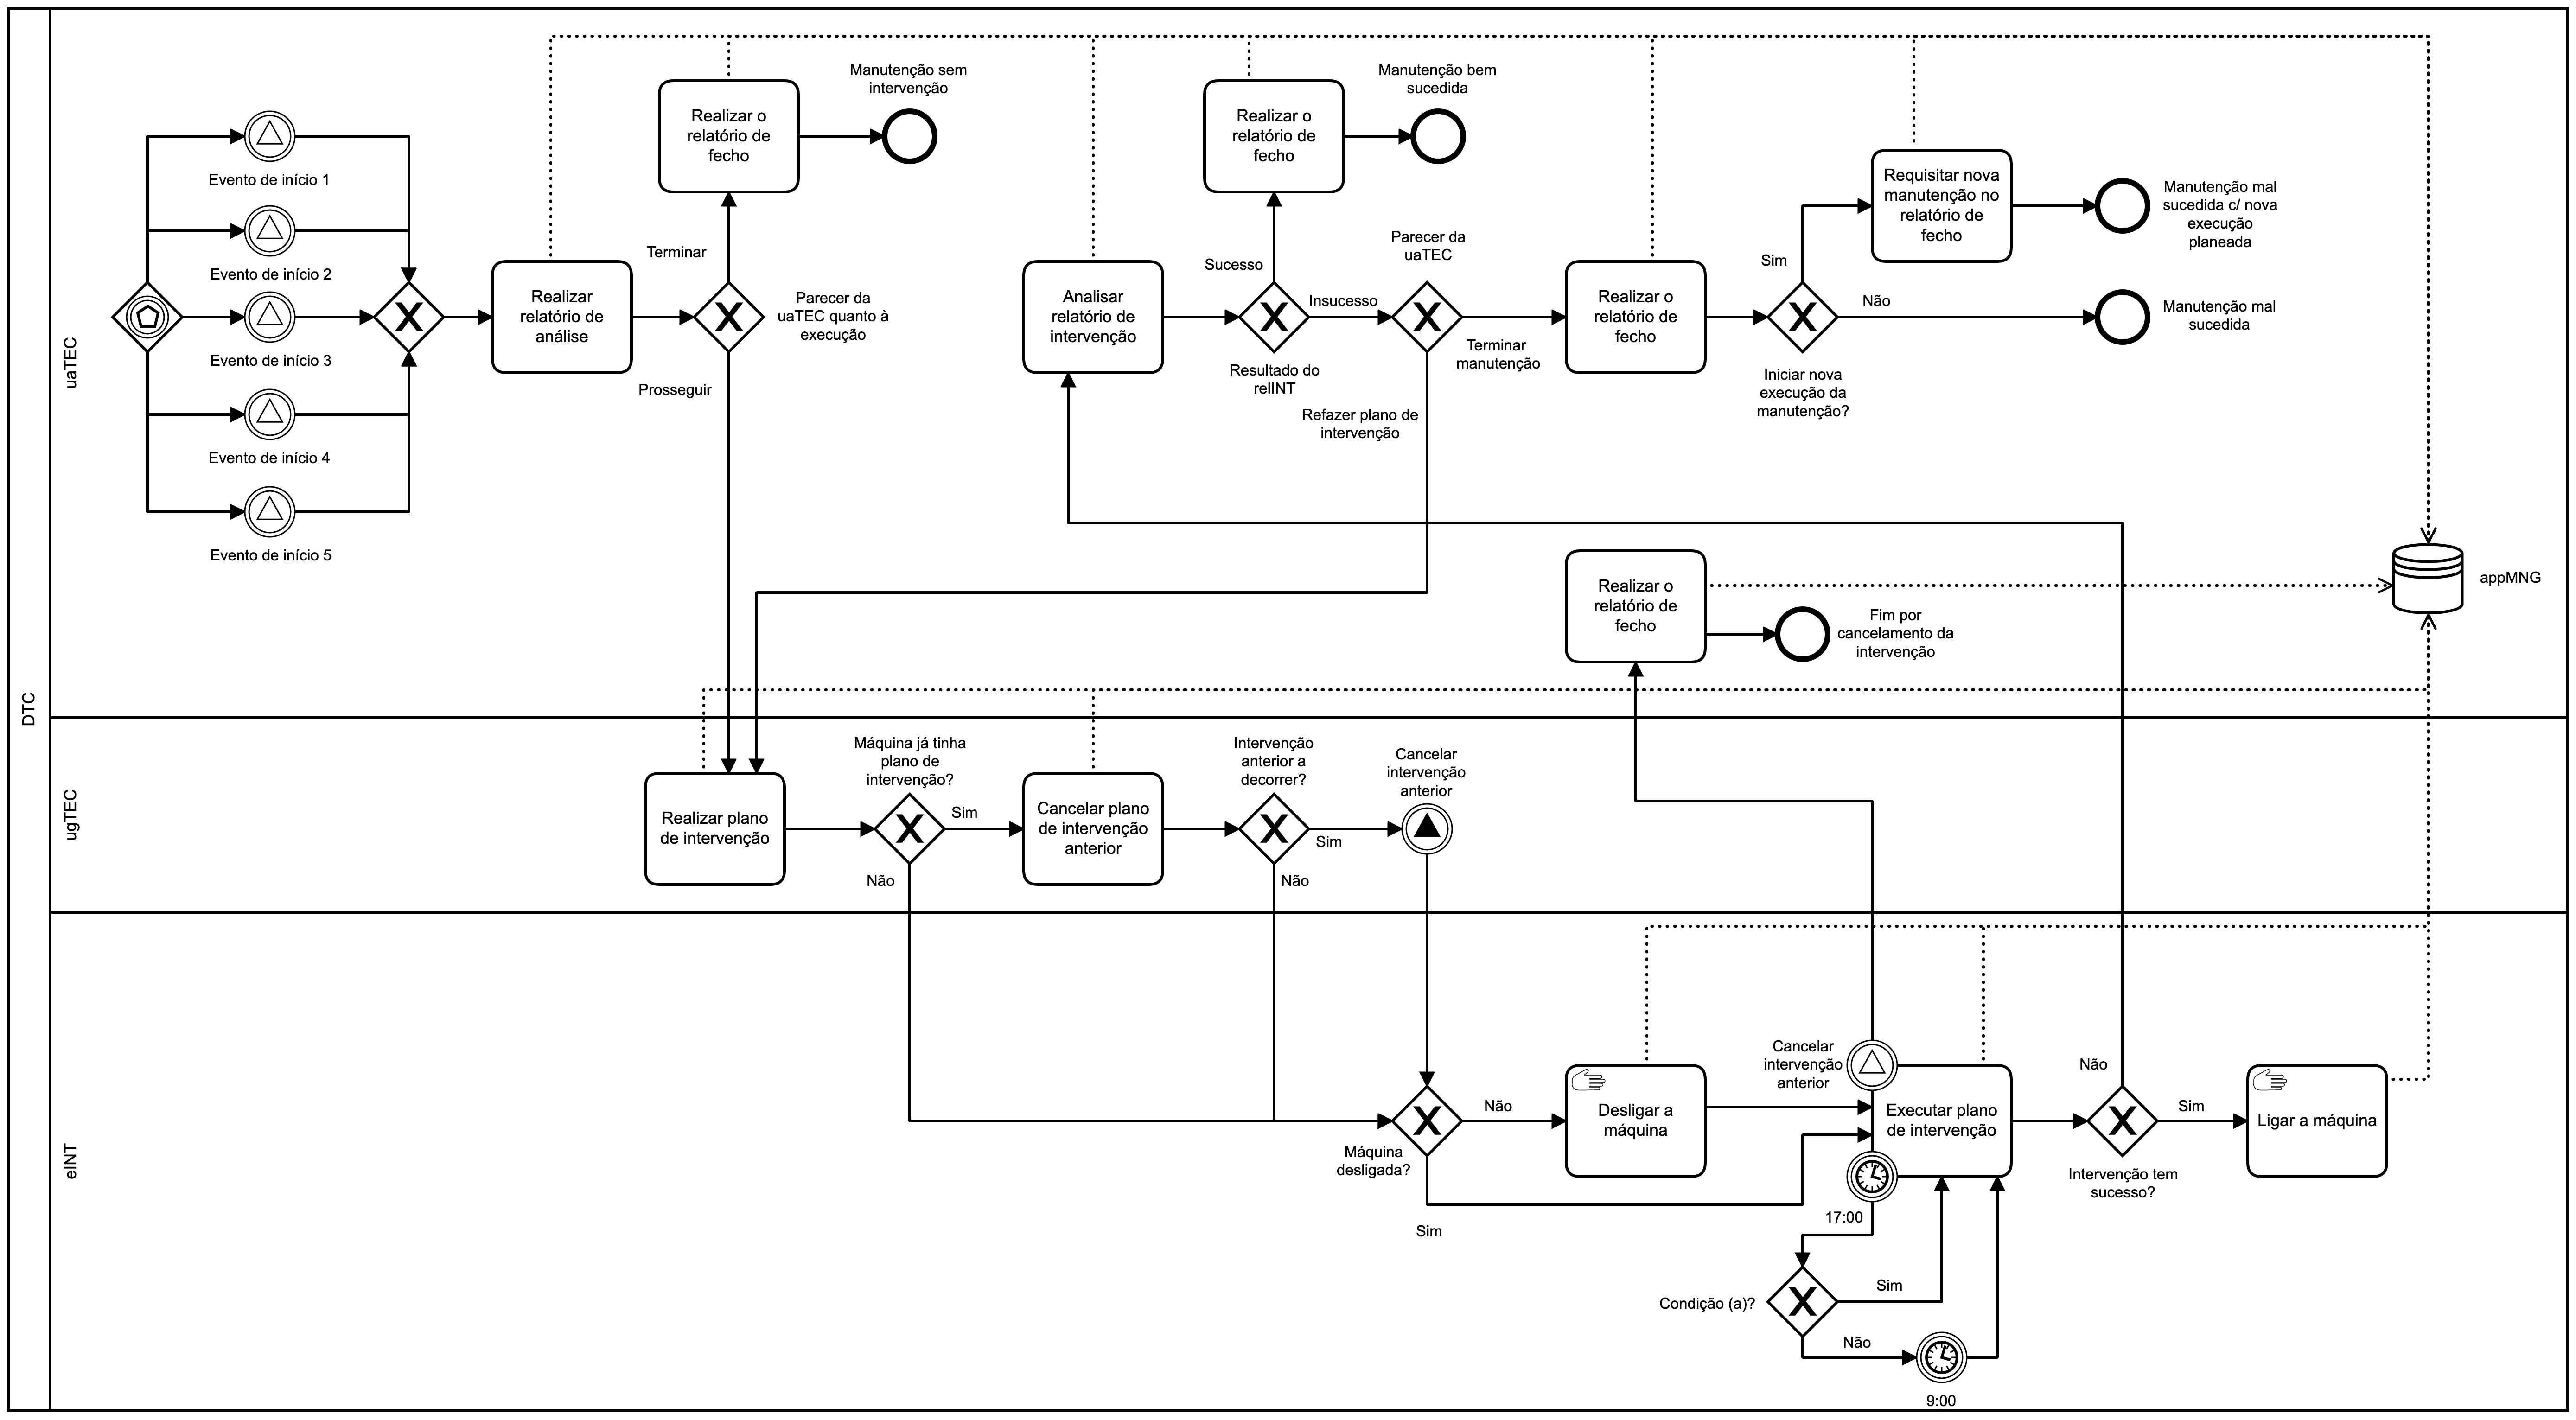
\includegraphics[angle=-90,origin=c, scale = 0.11]{one_pool.png}
    \end{figure}

    \pagebreak


    \begin{figure}[H]
        \centering
        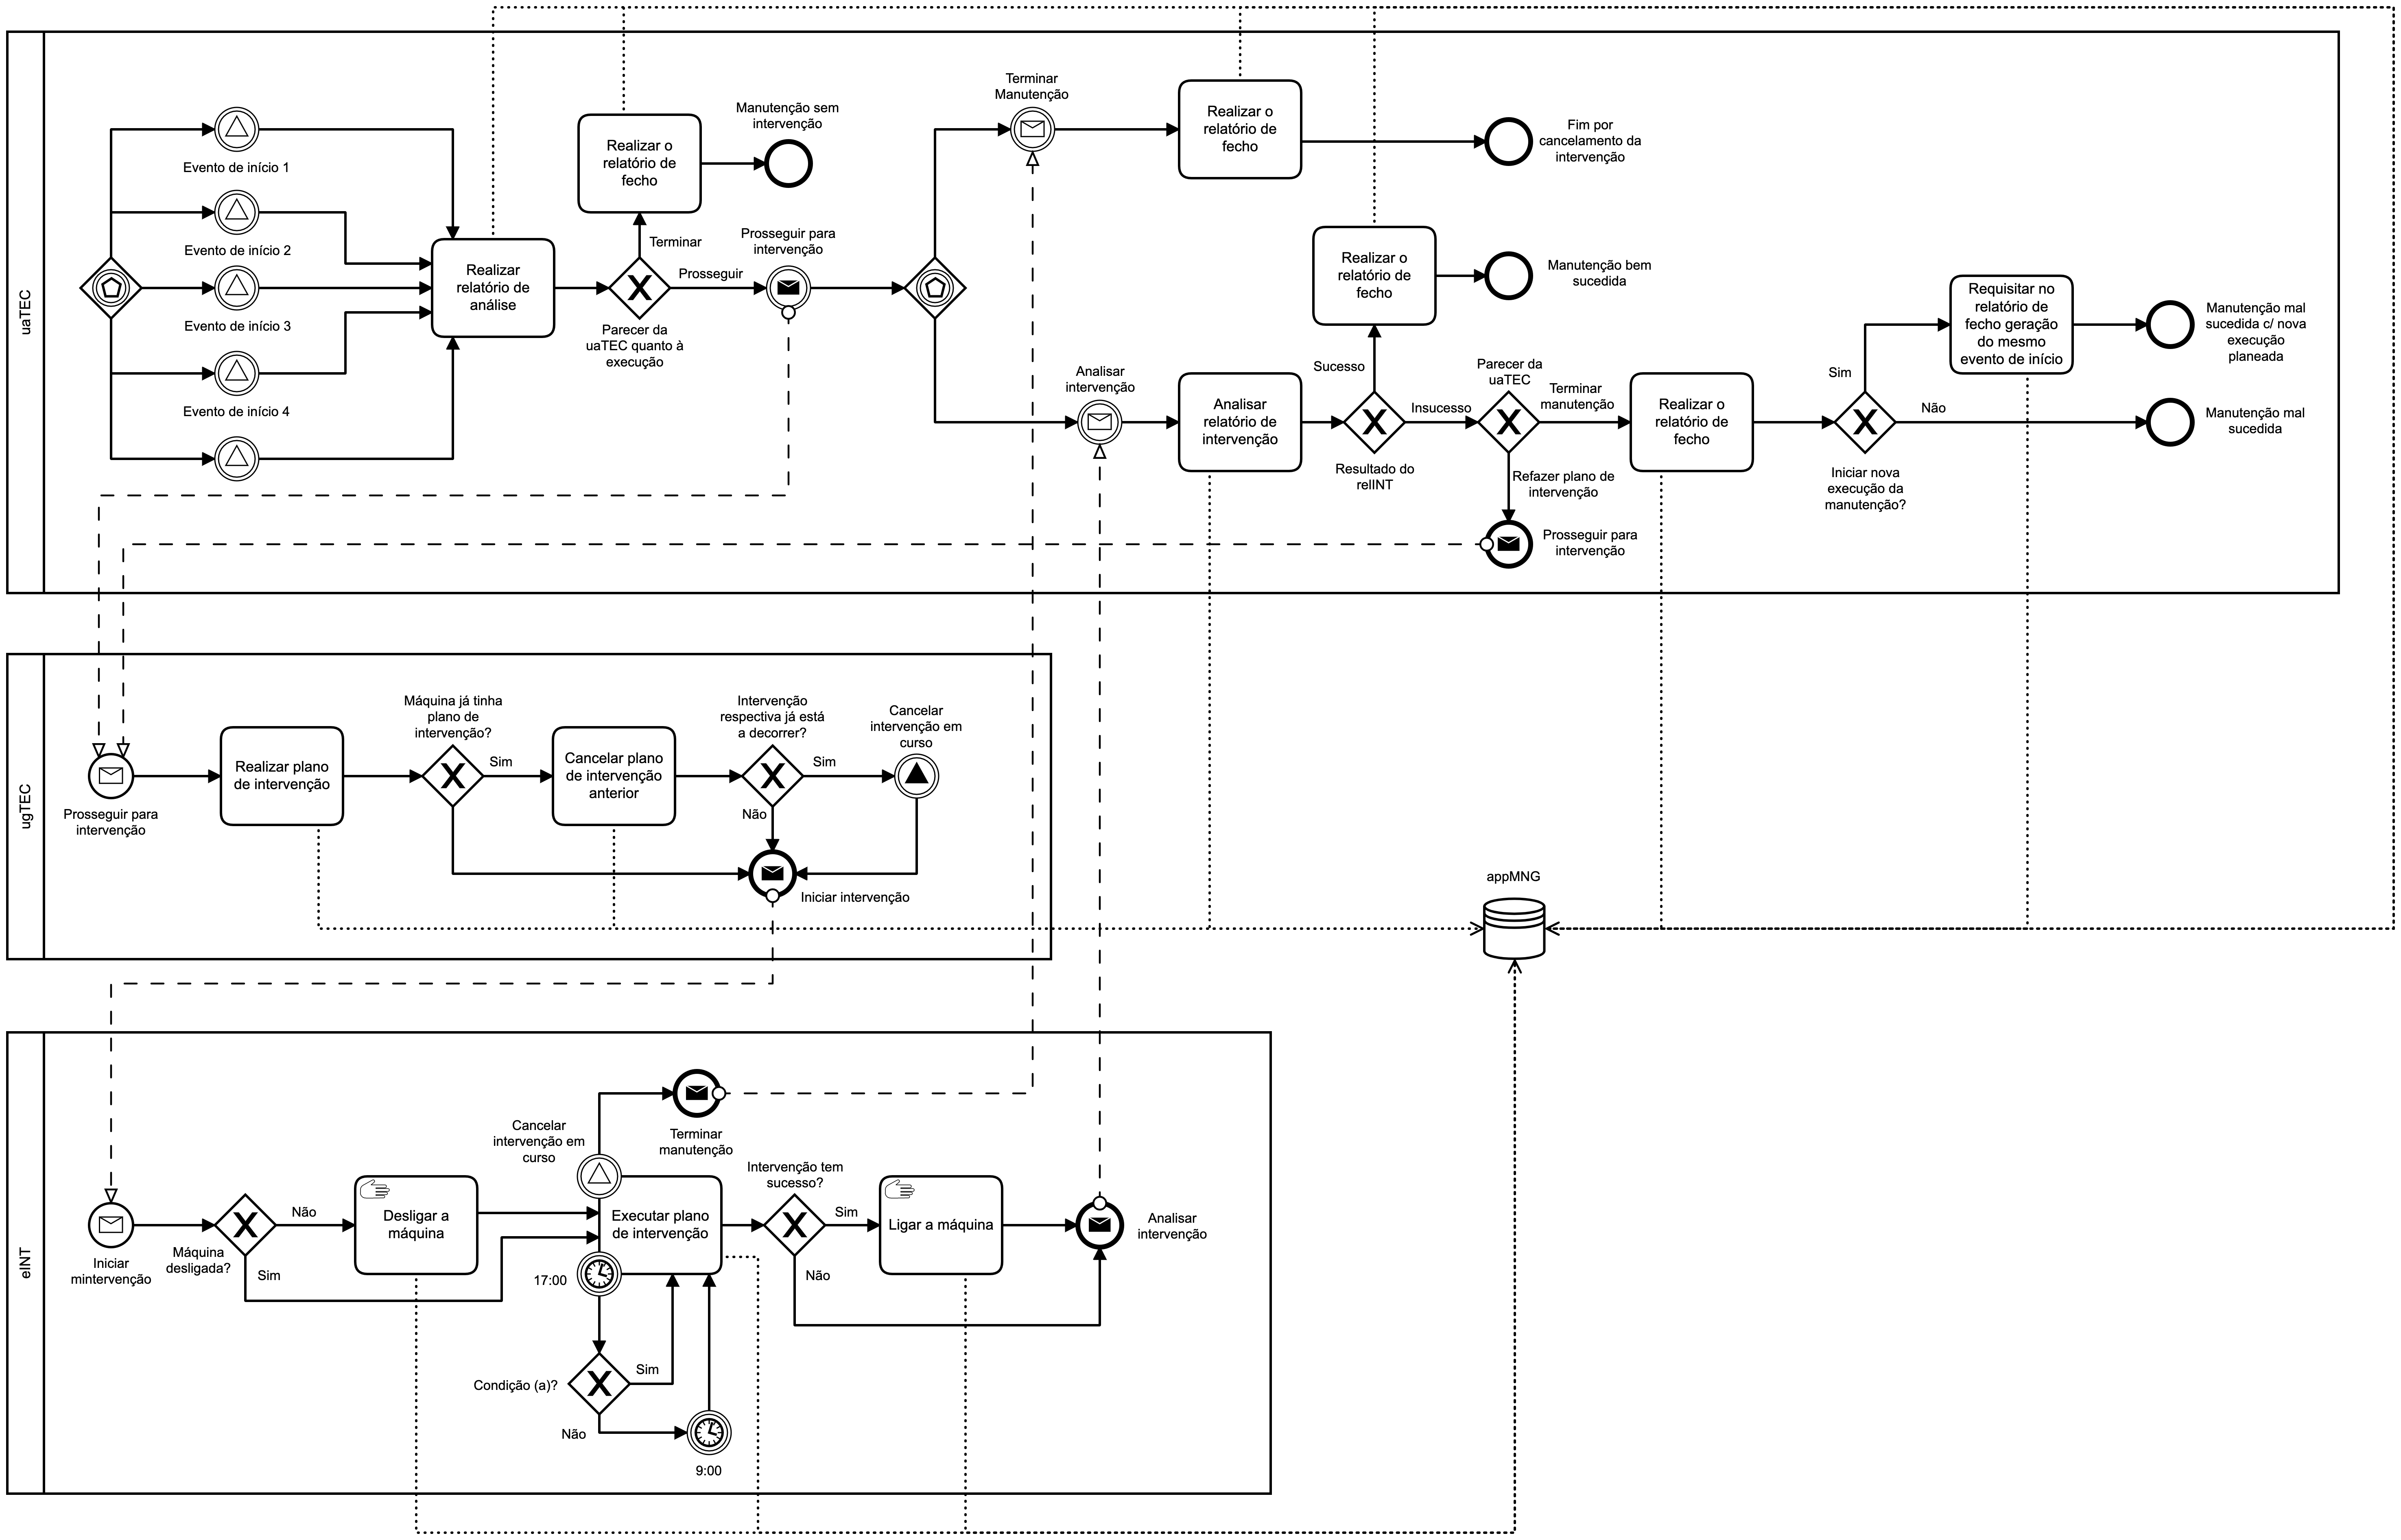
\includegraphics[angle=-90,origin=c, scale = 0.11]{various_pools.png}
    \end{figure}

\end{document}